\documentclass{article}


% if you need to pass options to natbib, use, e.g.:
%     \PassOptionsToPackage{numbers, compress}{natbib}
% before loading neurips_2024


% ready for submission
%  \usepackage{neurips_2024}


% to compile a preprint version, e.g., for submission to arXiv, add add the
% [preprint] option:
\usepackage[preprint]{neurips_2024}


% to compile a camera-ready version, add the [final] option, e.g.:
% \usepackage[final]{neurips_2024}


% to avoid loading the natbib package, add option nonatbib:
%    \usepackage[nonatbib]{neurips_2024}

\usepackage{natbib}
\usepackage[utf8]{inputenc} % allow utf-8 input
\usepackage[T1]{fontenc}    % use 8-bit T1 fonts
\usepackage{hyperref}       % hyperlinks
\usepackage{url}            % simple URL typesetting
\usepackage{booktabs}       % professional-quality tables
\usepackage{amsfonts}       % blackboard math symbols
\usepackage{amsmath}        % math environments
\usepackage{amssymb}        % additional math symbols including \oplus
\usepackage{nicefrac}       % compact symbols for 1/2, etc.
\usepackage{microtype}      % microtypography
\usepackage{xcolor}         % colors
\usepackage[pdftex]{graphicx}
\usepackage{multirow}
\usepackage{float}          % for [H] float placement


\title{Multi-Agent Learning Management System Assistant: An MCP-Based Framework for Intelligent Course Management Using AWS Bedrock}


% The \author macro works with any number of authors. There are two commands
% used to separate the names and addresses of multiple authors: \And and \AND.
%
% Using \And between authors leaves it to LaTeX to determine where to break the
% lines. Using \AND forces a line break at that point. So, if LaTeX puts 3 of 4
% authors names on the first line, and the last on the second line, try using
% \AND instead of \And before the third author name.


\author{%
   Pradhyumna Nagaraja Holla \\
  % examples of more authors
  % \And
  % Coauthor \\
  % Affiliation \\
  % Address \\
 \texttt{pnagaraj@stevens.edu} \\
 \texttt{\url{https://github.com/PradHolla/canvasXmcp}}
  % \AND
  % Coauthor \\
  % Affiliation \\
  % Address \\
  % \texttt{email} \\
  % \And
  % Coauthor \\
  % Affiliation \\
  % Address \\
  % \texttt{email} \\
  % \And
  % Coauthor \\
  % Affiliation \\
  % Address \\
  % \texttt{email} \\
}


\begin{document}


\maketitle

\section{Introduction}

Students managing multiple courses face significant challenges tracking assignments, deadlines, and academic content across Learning Management Systems (LMS) like Canvas. This project develops an intelligent conversational assistant using the Model Context Protocol (MCP) and Large Language Models (LLMs) via AWS Bedrock to automate student interactions with Canvas LMS.

Recent research demonstrates that AI agentic workflows including reflection, planning, tool use, and multi-agent collaboration offer promising solutions for educational innovation \cite{education2025agentic}. Wang et al. \cite{wang2025megaagent} introduced MegaAgent, showing that autonomous multi-agent systems can handle complex tasks without predefined procedures through dynamic task decomposition. The Model Context Protocol, as surveyed by recent work \cite{mcp2025landscape, mcp2025survey}, provides standardized interfaces for agent communication and context management, addressing critical limitations in LLM systems \cite{mcpenhance2025}.

Educational AI applications are emerging as transformative tools. Research on agentic workflows in education \cite{education2025agentic} highlights how specialized agents can personalize learning experiences. Work on integrating generative-conversational AI into LMS platforms \cite{lms2025ai} demonstrates the feasibility of such systems. However, practical implementations remain limited, particularly for student-facing applications that integrate real-time Canvas data through conversational interfaces with proper memory management and tool orchestration.

\subsection{Progress Summary}

This project has achieved significant milestones in developing a production-ready Canvas LMS assistant. The system architecture has evolved from the initial multi-agent proposal to a streamlined single-agent ReAct framework leveraging LangGraph for state management and MCP for standardized tool access. Key accomplishments include:

\textbf{Core Infrastructure (Weeks 1-2):}
\begin{itemize}
    \item Complete Canvas REST API client implementation supporting all student-accessible endpoints (courses, assignments, grades, quizzes, announcements, files)
    \item AWS Bedrock integration with ChatBedrockConverse supporting both Meta LLaMA 4 Maverick and OpenAI GPT-OSS models
    \item MCP server implementation using FastMCP with 9 specialized tools for Canvas data access
    \item LangGraph-based ReAct agent with conversational memory using MemorySaver checkpointing
\end{itemize}

\textbf{System Development (Weeks 3-5):}
\begin{itemize}
    \item Chainlit web interface providing real-time conversational interactions
    \item Token usage tracking and cost monitoring infrastructure
    \item Comprehensive testing framework with automated test runners for model evaluation
    \item Text sanitization utilities addressing Unicode handling issues in model outputs
\end{itemize}

\textbf{Evaluation Framework (Weeks 6-7):}
\begin{itemize}
    \item Systematic testing infrastructure supporting 149 queries across 4 test scenarios
    \item Streamlit-based manual evaluation application for human quality assessment
    \item Comparative analysis between LLaMA 4 Maverick and GPT-OSS 120B models
    \item Three-dimensional rating system (correctness, completeness, clarity) with failure type categorization
\end{itemize}

\subsection{Key Findings and Insights}

Through extensive testing and evaluation, several critical insights emerged:

\textbf{Architecture Simplification:} The initial multi-agent architecture was refined to a single ReAct agent with tool access, proving more effective for this domain. The unified agent architecture eliminates inter-agent coordination overhead while maintaining modularity through MCP-based tools. This aligns with recent findings that carefully designed single-agent systems can match multi-agent performance on structured tasks \cite{chen2024llmma}.

\textbf{Model Performance Disparities:} Comparative evaluation revealed distinct performance profiles: GPT-OSS 120B achieved 87.9\% pass rate (8.22/10 average score) versus LLaMA 4 Maverick's 76.5\% pass rate (6.84/10 average). Surprisingly, GPT-OSS proved both higher quality AND 19\% cheaper per query, 
eliminating the typical cost-quality tradeoff and making deployment decisions straightforward.

\textbf{Memory Management Trade-offs:} Testing revealed counterintuitive memory effects: GPT-OSS improved dramatically with conversation memory (+2.46 points, 98\% pass rate), while LLaMA performance degraded slightly (-0.31 points). This suggests fundamental differences in how models leverage conversational context, with implications for production deployment strategies.

\textbf{Systematic Failure Patterns:} Analysis of 53 total failures across both models revealed distinct failure modes: LLaMA's primary issue was error handling (46\% of failures exposed raw code/tool outputs), while GPT-OSS suffered from wrong data retrieval (56\% of failures returned data from incorrect courses). These patterns inform targeted improvement strategies.

\subsection{Challenges Addressed}

\textbf{Technical Challenges:}
\begin{itemize}
    \item \textit{Token Accounting Bug:} Initial implementation incorrectly summed usage metadata across conversation history, reporting 1.9M tokens for queries actually using 45K tokens. Fixed by tracking only latest AIMessage metadata.
    \item \textit{GPT-OSS Unicode Issues:} Model generated \texttt{\textbackslash u202f} and \texttt{\textbackslash u2013} characters causing tokenization errors. Implemented TextSanitizer utility for comprehensive Unicode normalization.
    \item \textit{Course ID Resolution:} Both models struggled with course name to ID mapping, causing 23 instances of wrong data retrieval. Addressed through improved prompting and explicit tool naming conventions.
    \item \textit{Temporal Query Failures:} Both models defaulted to 7-day windows, failing 80\% of temporal queries like "deadlines for November." Requires future work on date parsing and dynamic parameter handling.
\end{itemize}

\textbf{Methodological Challenges:}
\begin{itemize}
    \item \textit{Evaluation Framework Design:} Automated metrics (latency, token usage, cost) failed to capture critical quality issues like code exposure and hallucinations. Developed comprehensive manual evaluation methodology with three-dimensional scoring and failure categorization, evaluating all 149 queries manually.
    \item \textit{Memory Testing Complexity:} Separating memory effects from model capability required parallel test suites (with/without memory) using identical query sets, revealing memory as a double-edged sword depending on model architecture.
\end{itemize}

The system is now in a production-ready state with a robust evaluation methodology, ready for final refinements and deployment planning in the remaining project weeks.


\section{Problem Formulation}

This project implements a conversational question-answering and tool-use system \cite{chen2024llmma} for Canvas LMS data access. The task combines information retrieval, multi-turn dialogue management, and structured action execution through a ReAct agent architecture \cite{yao2023react}.

\subsection{Formal Task Definition}

\textbf{Input Space:} Let $\mathcal{Q}$ denote the space of natural language queries from students. Let $\mathcal{C}$ represent Canvas LMS data including courses $C = \{c_1, ..., c_n\}$, assignments $A = \{a_1, ..., a_m\}$, grades $G$, quizzes $Q$, and announcements $N$. Let $\mathcal{H}$ denote conversation history $H = \{(q_1, r_1), ..., (q_t, r_t)\}$ where $q_i \in \mathcal{Q}$ and $r_i \in \mathcal{R}$ are query-response pairs.

\textbf{Output Space:} The system produces responses $r \in \mathcal{R}$ in natural language, along with potential tool invocations $\mathcal{T} = \{t_1, ..., t_k\}$ where each $t_i: \mathcal{C} \rightarrow \mathcal{D}$ maps Canvas data to structured results.

\textbf{Agent Function:} The ReAct agent implements a function $f: \mathcal{Q} \times \mathcal{H} \times \mathcal{C} \rightarrow \mathcal{R} \times \mathcal{T}$ that maps current query, conversation history, and Canvas context to natural language responses and tool executions.

The agent operates through iterative reasoning:
\begin{equation}
f(q_t, H, C) = \text{LLM}(\text{prompt}(q_t, H) \oplus \text{tools}(\mathcal{T}))
\end{equation}

where $\oplus$ denotes tool-augmented generation, allowing the LLM to interleave reasoning steps with tool calls.

\subsection{Task Categorization}

This system addresses multiple interconnected tasks:

\begin{enumerate}
\item \textbf{Information Retrieval:} Given query $q$ requesting Canvas data (e.g., ``What courses am I taking?''), retrieve relevant subset $D \subseteq \mathcal{C}$ via tool invocations and format as natural language response.

\item \textbf{Multi-Turn Dialogue:} Maintain conversation context $H$ to resolve references across turns (e.g., ``What's due in my second course?'' following ``What courses am I taking?''), requiring coreference resolution and context tracking.

\item \textbf{Temporal Reasoning:} Parse temporal expressions (``this week,'' ``by Friday,'' ``November deadlines'') into structured date queries for filtering assignments and deadlines.

\item \textbf{Aggregation and Synthesis:} Combine data from multiple courses (e.g., ``Show all my grades'') requiring orchestration of multiple tool calls and result aggregation.

\item \textbf{Complex Query Decomposition:} Break down multi-step queries (e.g., ``Which course needs the most attention?'') into constituent retrieval and reasoning steps.
\end{enumerate}

\subsection{Evaluation Framework}

\textbf{Automated Metrics:}
\begin{itemize}
\item \textit{Response Latency:} Time $\Delta t$ from query submission to response generation
\item \textit{Token Efficiency:} Input tokens $T_{in}$ and output tokens $T_{out}$ per query
\item \textit{Cost:} $\text{Cost} = (T_{in} \times p_{in} + T_{out} \times p_{out})/1000$ where $p_{in}, p_{out}$ are per-1K token prices
\item \textit{Tool Usage:} Number of tool invocations $|\mathcal{T}|$ and tool call correctness
\end{itemize}

\textbf{Human Evaluation Metrics:}

For each query $q_i$ with model response $r_i$, human evaluators (which is just myself) assign scores:
\begin{equation}
S(r_i) = \frac{1}{3}(S_{\text{correct}}(r_i) + S_{\text{complete}}(r_i) + S_{\text{clear}}(r_i))
\end{equation}

where each dimension $S_* \in [1, 10]$ and responses with $S(r_i) < 6$ are classified as failures with associated failure type $f_i \in \{\text{wrong\_data}, \text{incomplete}, \text{error\_handling}, \text{hallucination}, ...\}$.

\textbf{Comparative Evaluation:}

Let $M_1$ (LLaMA 4 Maverick) and $M_2$ (GPT-OSS 120B) denote the two evaluated models. For query set $\mathcal{Q}_{\text{test}}$ with $|\mathcal{Q}_{\text{test}}| = 149$:

\begin{itemize}
\item \textit{Pass Rate:} $P(M_i) = \frac{1}{|\mathcal{Q}_{\text{test}}|} \sum_{q \in \mathcal{Q}_{\text{test}}} \mathbb{1}[S(M_i(q)) \geq 6]$
\item \textit{Category Performance:} For each category $c \in \{\text{simple}, \text{course}, \text{temporal}, ...\}$, compute $S_c(M_i) = \frac{1}{|\mathcal{Q}_c|} \sum_{q \in \mathcal{Q}_c} S(M_i(q))$
\item \textit{Cost-Quality Ratio:} $\text{CQR}(M_i) = \frac{\sum_{q} S(M_i(q))}{\sum_{q} \text{Cost}(M_i(q))}$ measuring score per dollar
\end{itemize}

\subsection{Memory-Augmented Setting}

The system operates in two configurations:

\textbf{Stateless:} Each query $q_t$ processed independently with $f(q_t, \emptyset, C)$, evaluating raw model capability.

\textbf{Stateful:} Queries processed with full conversation history $f(q_t, H_{1:t-1}, C)$, testing context retention and multi-turn coherence.

Performance delta $\Delta_{\text{memory}}(M_i) = S_{\text{memory}}(M_i) - S_{\text{no-memory}}(M_i)$ quantifies memory benefit, with observed results showing $\Delta_{\text{memory}}(\text{GPT-OSS}) = +2.46$ while $\Delta_{\text{memory}}(\text{LLaMA}) = -0.31$, revealing fundamental architectural differences.

This formulation enables systematic evaluation of conversational AI systems for educational applications, combining quantitative performance metrics with qualitative human assessment to capture both technical efficiency and real-world utility.

\section{Methods}

This section describes the implemented system architecture, technical decisions, and rationale for the approaches taken. The system evolved from the initially proposed multi-agent architecture to a streamlined ReAct agent design leveraging modern LLM orchestration frameworks.

\subsection{Architecture Overview}

\textbf{Design Philosophy:} The final architecture adopts a single-agent ReAct (Reasoning and Acting) paradigm \cite{yao2023react} rather than the initially proposed multi-agent system. This decision was driven by several factors: (1) reduced coordination complexity, (2) simplified state management, (3) more predictable behavior, and (4) easier debugging and testing. The ReAct pattern enables the agent to interleave reasoning steps with tool invocations, effectively achieving the modularity of multi-agent systems while avoiding inter-agent communication overhead.

\textbf{Core Components:}
\begin{itemize}
    \item \textit{Canvas API Client} (\texttt{src/canvas/client.py}): Comprehensive REST API wrapper handling authentication, rate limiting, and error handling
    \item \textit{MCP Server} (\texttt{src/mcp/canvas\_server.py}): FastMCP-based tool server exposing 9 Canvas operations as standardized MCP tools \cite{mcp2025landscape}
    \item \textit{ReAct Agent} (\texttt{src/agent/canvas\_agent.py}): LangGraph-based orchestrator managing LLM interactions, tool calls, and conversation state
    \item \textit{Chainlit Interface} (\texttt{app.py}): Web-based conversational UI with real-time streaming and token tracking
    \item \textit{Testing Framework} (\texttt{tests/}): Automated test runners and Streamlit-based manual evaluation system
\end{itemize}

\begin{figure}[h]
\centering

\includegraphics[width=0.9\textwidth]{canvasXmcp.jpg}
\caption{System Architecture}
\label{fig:architecture}
\end{figure}

Figure~\ref{fig:architecture} illustrates the complete system architecture, showing the interaction flow between the user interface (Chainlit), the ReAct agent (LangGraph), the MCP server, and the Canvas LMS API with AWS Bedrock.

\subsection{Canvas API Integration}

The Canvas client implements a complete wrapper around Canvas LMS REST API v1 endpoints relevant to student workflows. Key implementation details:

\textbf{Authentication:} OAuth2 bearer token authentication using personal access tokens stored in environment variables. All requests include \texttt{Authorization: Bearer <token>} headers.

\textbf{Supported Endpoints:}
\begin{itemize}
    \item \texttt{GET /api/v1/courses}: Retrieve enrolled courses with enrollment states
    \item \texttt{GET /api/v1/courses/\{id\}/assignments}: Fetch course assignments with submission status
    \item \texttt{GET /api/v1/courses/\{id\}/quizzes}: Access quiz metadata and student submissions
    \item \texttt{GET /api/v1/courses/\{id\}/assignment\_groups}: Retrieve grade weighting information
    \item \texttt{GET /api/v1/courses/\{id\}/announcements}: Fetch recent course announcements
    \item \texttt{GET /api/v1/users/self/upcoming\_events}: Access calendar events with date filtering
\end{itemize}

\textbf{Rate Limiting:} Canvas enforces 3000 requests per hour per user. The client implements request throttling using Python's \texttt{time.sleep()} with exponential backoff on 429 status codes. No explicit caching layer was implemented at this stage, as query patterns during testing showed <10 API calls per user session, well within rate limits.

\textbf{Performance Optimization Through Caching:}

Initial implementation suffered from N+1 query problem: fetching upcoming assignments across 5 courses required 6 sequential API calls (\texttt{get\_courses()} + 5x \texttt{get\_assignments()}), resulting in 5-6 second response times. Implemented tiered caching strategy:

\begin{itemize}
    \item Course metadata: 5-minute TTL (time-to-live)
    \item Assignments: 5-minute TTL with per-course invalidation
    \item Announcements: 2-minute TTL (more time-sensitive)
\end{itemize}

Cache hit rate reached 83\% after warmup, reducing API calls by 85\% and average response time from 5.6s to 1.8s. This aggressive caching proved critical for staying within Canvas's 3000 requests/hour rate limit during development and testing phases.


\textbf{Error Handling:} All API calls wrapped in try-except blocks catching \texttt{requests.exceptions} (network errors, timeouts) and HTTP error codes (401 unauthorized, 404 not found, 500 server errors). Error responses sanitized before presentation to users, preventing raw JSON exposure.

\textbf{Data Preprocessing:} Assignment due dates converted from ISO8601 strings to Python \texttt{datetime} objects. Grades normalized to 0-100 scale. HTML content in announcements stripped using regex patterns. This preprocessing ensures consistent data types for LLM consumption.

\textbf{Canvas API Quirks Discovered During Implementation:}

Real-world Canvas deployment revealed several API inconsistencies requiring custom handling logic:

\textit{Dual Quiz Systems:} Canvas supports both native quizzes (\texttt{submission\_type: "online\_quiz"}) and LTI external tool quizzes (\texttt{is\_quiz\_lti\_assignment: true}). CS 555 (Agile Methods) uses LTI quizzes appearing only in the assignments endpoint, causing \texttt{get\_quizzes()} to return empty results. Implemented unified detection checking both quiz types plus name pattern matching to capture all quiz formats.

\textit{Module Organization Inconsistency:} Not all courses use Canvas modules feature. CS 584 (NLP) organizes content exclusively through files, causing \texttt{get\_modules()} failures. Added automatic fallback logic: when no modules exist, system formats files as pseudo-modules maintaining consistent structure for students.

\textit{Submission Status Unreliability:} The \texttt{has\_submitted\_submissions} flag proved unreliable for actual submission verification. Resolved by adding \texttt{include[]=submission} parameter to retrieve actual submission objects rather than relying on boolean flags.

\textit{Timezone Handling:} Canvas returns UTC timestamps with 'Z' suffix, causing deadline confusion (``11:59 PM'' displayed as ``3:59 AM''). Implemented \texttt{datetime.astimezone()} conversion ensuring all displayed times use user's local timezone.

These discoveries highlight the importance of testing against production data rather than synthetic examples, as LMS implementations vary significantly across institutions and courses.


\subsection{Model Context Protocol (MCP) Implementation}

The system leverages FastMCP \cite{mcp2025landscape}, a lightweight Python implementation of Anthropic's Model Context Protocol, to standardize tool interfaces. This design decision enables potential future migration to alternative LLM providers or frameworks with minimal refactoring.

\textbf{Tool Definitions:} Nine MCP tools implemented, each with typed parameters and structured return values:

\begin{enumerate}
    \item \texttt{get\_courses()}: Returns list of enrolled courses with IDs, names, and enrollment status
    \item \texttt{get\_upcoming\_assignments(days: int = 7)}: Fetches assignments due within specified window
    \item \texttt{get\_assignments(course\_id: str)}: Retrieves all assignments for a specific course
    \item \texttt{get\_quizzes(course\_id: str)}: Returns quiz metadata, scores, and submission timestamps
    \item \texttt{get\_grades(course\_id: str)}: Calculates current grade and component breakdown
    \item \texttt{get\_all\_grades()}: Aggregates grades across all enrolled courses
    \item \texttt{get\_course\_summary(course\_id: str)}: Comprehensive course overview combining multiple data sources
    \item \texttt{get\_announcements(days: int = 7)}: Fetches recent announcements with date filtering
    \item \texttt{get\_course\_id\_by\_name(course\_name: str)}: Resolves course names to numeric IDs
\end{enumerate}

\textbf{Course Name Resolution Challenge:}

Early testing revealed systematic failures on queries like ``What's due in Machine Learning?'' The root cause: MCP tools accept only numeric course IDs (e.g., 80546), but users naturally reference courses by name. Initial prompt attempted to have the LLM remember name-to-ID mappings from previous \texttt{get\_courses()} calls, but this proved unreliable across conversation turns.

Solution required adding dedicated \texttt{get\_course\_id\_by\_name(course\_name: str)} tool performing fuzzy matching against enrolled courses. Updated system prompt with explicit guidance:

\begin{verbatim}
IMPORTANT: Canvas APIs need numeric course IDs.
If user mentions course by name, call 
get_course_id_by_name() FIRST, then use 
returned ID for subsequent tool calls.
\end{verbatim}

This architectural decision, exposing name resolution as explicit tool rather than hidden logic-reduced wrong course data errors by 60\% in subsequent testing.


\textbf{Tool Server Architecture:} The MCP server runs as a subprocess spawned by the main agent process via \texttt{stdio\_client}. Communication uses JSON-RPC over standard input/output streams, avoiding network sockets and simplifying deployment. The server initializes once per session, maintaining a persistent Canvas API client connection.

\textbf{Pydantic Validation:} All tool parameters validated using Pydantic models, ensuring type safety and providing automatic JSON schema generation for LLM tool calling. Invalid parameters caught before Canvas API invocation, reducing unnecessary network requests.

\subsection{LLM Integration and ReAct Agent}

\textbf{Model Selection:} AWS Bedrock serves as the LLM backend, providing access to multiple foundation models without managing infrastructure. Two models evaluated:

\begin{itemize}
    \item \textit{Meta LLaMA 4 Maverick 17B} (\texttt{us.meta.llama4-maverick-17b-instruct-v1:0}): Cost-effective option at \$0.00027 input / \$0.00032 output per 1K tokens
    \item \textit{OpenAI GPT-OSS 120B} (\texttt{openai.gpt-oss-120b-1:0}): Higher quality option at \$0.000165 input / \$0.00066 output per 1K tokens
\end{itemize}

Model selection initially favored LLaMA for development cost savings, with GPT-OSS evaluated for production quality comparison. Bedrock integration via \texttt{ChatBedrockConverse} enables streaming responses for real-time UI updates.

\textbf{ReAct Agent Implementation:} LangGraph's \texttt{create\_react\_agent()} function constructs the agent graph with automatic tool calling support. The agent follows this execution loop:

\begin{enumerate}
    \item Receive user query and conversation history
    \item LLM generates reasoning step or tool invocation
    \item If tool call: execute tool, append result to context, return to step 2
    \item If final answer: generate natural language response and terminate
\end{enumerate}

\textbf{Recursion Limit Tuning:}

LangGraph's default recursion limit of 25 proved insufficient for complex multi-step queries. Queries like ``Which course needs the most attention?'' require tool calls for grades, assignments, and temporal filtering, often exceeding limit before reaching stopping condition. This manifested as:

\begin{verbatim}
RecursionError: Recursion limit of 25 reached 
without hitting a stop condition.
\end{verbatim}

Increased limit to 50 and added explicit stopping conditions to system prompt:
\begin{itemize}
    \item Generate final answer when sufficient data retrieved
    \item Avoid redundant tool calls for already-fetched data
    \item Terminate after 3 consecutive tool failures
\end{itemize}

Post-adjustment, 95\% of queries completed within 10 iterations, with complex queries averaging 15 iterations. The 50-iteration limit provides safety margin without enabling infinite loops.

\textbf{Prompt Engineering:} System prompt carefully crafted to enforce behavior constraints:

\begin{verbatim}
You are a Canvas LMS assistant helping students.

TOOLS:
- get_courses() - enrolled courses
- get_upcoming_assignments(days=7) - assignments due soon
[... tool descriptions ...]

RULES:
1. Use tools to get real data
2. Format dates as "October 23, 2025"
3. Format scores as "8.5/10"
4. Never show course IDs or technical details
5. Be concise and helpful
6. NEVER output code (Python, JSON, etc.)

IMPORTANT: Canvas APIs need numeric course IDs.
If user mentions course by name, call 
get_course_id_by_name() first.

Present information cleanly with bullet points.
No raw JSON. No code.
\end{verbatim}

\textbf{Prompt Evolution Through Testing:}

Initial system prompt exceeded 50 lines with detailed instructions for each tool, edge case handling, and formatting guidelines. Testing revealed this complexity confused the agent, particularly on queries like ``What's due this week?'' where tool selection became inconsistent.

Iteratively refined prompt through 3 major revisions:
\begin{enumerate}
    \item \textit{Version 1 (50+ lines):} Comprehensive but overwhelming, 65\% tool selection accuracy
    \item \textit{Version 2 (35 lines):} Simplified instructions, improved to 78\% accuracy
    \item \textit{Version 3 (20 lines):} Focused on essential rules with clear tool descriptions, achieved 89\% accuracy
\end{enumerate}

Final prompt follows ``less is more'' principle: concise rules, explicit tool capabilities, minimal edge case handling. Counter-intuitively, removing detailed instructions improved agent reasoning by reducing decision paralysis.


Temperature set to 0.3 to balance factual accuracy with natural language fluency. Lower temperatures (0.1-0.2) produced overly rigid responses, while higher values (>0.5) introduced occasional hallucinations.

\textbf{Conversation Memory:} LangGraph's \texttt{MemorySaver} checkpointer maintains conversation state across queries within a session. Each query assigned a unique \texttt{thread\_id}, enabling multi-turn dialogue with coreference resolution. Memory stored in-process (not persisted to disk), resetting on application restart. This design choice simplifies deployment while meeting the single-session use case requirement.

\subsection{Text Sanitization and Output Processing}

\textbf{Model-Specific Response Handling:}

Switching from LLaMA to GPT-OSS revealed fundamental differences in response structure requiring adaptive parsing:

\textit{LLaMA:} Returns simple string responses
\begin{verbatim}
"You have 3 assignments due this week..."
\end{verbatim}

\textit{GPT-OSS:} Returns structured list of content blocks
\begin{verbatim}
[
  {"type": "reasoning_content", 
   "reasoning_content": {"text": "..."}},
  {"type": "text", 
   "text": "You have 3 assignments..."}
]
\end{verbatim}

Implemented polymorphic response extractor checking \texttt{isinstance(content, list)} and handling both formats. This abstraction enables seamless model switching without code changes outside the parsing layer.

\textbf{Unicode Handling Challenge:} Initial testing revealed GPT-OSS generates Unicode escape sequences (\texttt{\textbackslash u202f} non-breaking spaces, \texttt{\textbackslash u2013} en-dashes) causing Bedrock tokenization errors. Implemented \texttt{TextSanitizer} utility applying normalization rules:

\begin{itemize}
    \item Replace \texttt{\textbackslash u202f} with regular spaces
    \item Convert \texttt{\textbackslash u2013}, \texttt{\textbackslash u2014} to ASCII hyphens
    \item Strip HTML tags from announcement content
    \item Normalize newlines to \texttt{\textbackslash n}
\end{itemize}

Applied to all model outputs before presentation, ensuring consistent rendering across different clients.

\textbf{Reasoning Visibility:} GPT-OSS embeds internal reasoning in separate \texttt{reasoning\_content} blocks invisible to users. While useful for debugging, exposing raw reasoning clutters conversational interface. Implemented Chainlit accordion component allowing optional reasoning expansion:

\begin{verbatim}
[Response]
You have 3 assignments due this week...

[Reasoning - Click to expand]
First, I'll fetch courses, then check 
assignments for each...
\end{verbatim}

This preserves transparency for interested users while maintaining clean default UX.

\subsection{Testing Infrastructure}

\textbf{Automated Test Framework:} Developed comprehensive testing system (\texttt{tests/test\_runner.py}, \texttt{tests/test\_runner\_with\_memory.py}) supporting:

\begin{itemize}
    \item Parallel model evaluation (LLaMA and GPT-OSS on identical query sets)
    \item Memory vs.\ no-memory comparisons using configurable checkpointing
    \item Per-query metrics tracking: latency, tokens (input/output), cost, tool calls
    \item JSON output for programmatic analysis
\end{itemize}

\textbf{Token Accounting Fix:} Initial implementation incorrectly accumulated \texttt{usage\_metadata} across conversation history, reporting 1.9M tokens for queries actually using 45K tokens. Fixed by extracting metadata only from latest \texttt{AIMessage}:

\begin{verbatim}
# Find latest AIMessage (current response)
for msg in reversed(result["messages"]):
    if msg.__class__.__name__ == 'AIMessage':
        total_input = msg.usage_metadata["input_tokens"]
        total_output = msg.usage_metadata["output_tokens"]
        break
\end{verbatim}

This correction critical for accurate cost projections and performance analysis.

\textbf{Manual Evaluation System:} Streamlit web application (\texttt{tests/evaluator\_app.py}) enables systematic human evaluation:

\begin{itemize}
    \item Side-by-side response comparison for each query
    \item Three-dimensional rating (correctness, completeness, clarity) on 1-10 scale
    \item Failure type categorization (wrong data, incomplete, error handling, hallucination, etc.)
    \item Notes field for qualitative observations
    \item Progress tracking and incremental saving
    \item Comprehensive JSON export with aggregate statistics
\end{itemize}

Evaluated all 149 queries manually, providing rich qualitative dataset complementing automated metrics.

\subsection{Deployment and User Interface}

\textbf{Chainlit Web Application:} Selected Chainlit framework for rapid prototyping of conversational UI. Advantages over alternatives (Streamlit, Gradio):

\begin{itemize}
    \item Native support for streaming LLM responses (real-time token-by-token display)
    \item Built-in conversation threading and message history
    \item Minimal boilerplate code (30 lines for complete interface)
    \item Automatic handling of async functions
\end{itemize}

\textbf{Cost Tracking:} Implemented real-time token and cost monitoring using custom \texttt{TokenTracker} class. Each query logs:

\begin{verbatim}
{
  "timestamp": "2025-11-03T14:23:45",
  "model_id": "us.meta.llama4-maverick-17b-instruct-v1:0",
  "input_tokens": 2847,
  "output_tokens": 156,
  "cost_usd": 0.000819,
  "query": "What courses am I taking?",
  "response_time": 1.34
}
\end{verbatim}

Session summaries display total tokens, total cost, and average cost per query, enabling budget tracking during development.

\subsection{Rationale for Technical Decisions}

\textbf{Why ReAct over Multi-Agent:} Initial proposal specified multi-agent architecture with specialized agents (router, Canvas data, summarizer, etc.). After initial prototyping, simplified to ReAct agent because:

\begin{enumerate}
    \item \textit{Task Simplification:} Canvas queries rarely require complex agent coordination. Most tasks solvable through 1-3 sequential tool calls.
    \item \textit{Debugging Complexity:} Multi-agent systems introduce failure modes from inter-agent communication, state synchronization, and coordination protocols. ReAct's linear execution easier to debug.
    \item \textit{Latency Overhead:} Each agent transition incurs LLM invocation. ReAct completes queries in single LLM session with multiple tool calls.
    \item \textit{State Management:} Single agent simplifies conversation memory. Multi-agent requires complex shared state or message passing.
\end{enumerate}

This aligns with recent findings that careful prompt engineering and tool design can match multi-agent performance on structured domains \cite{chen2024llmma}.

\textbf{Why Bedrock over OpenAI API:} AWS Bedrock chosen for:

\begin{enumerate}
    \item Access to multiple model families (Meta, Anthropic, Amazon) through single API
    \item Pay-per-use pricing without subscriptions or commitments
    \item No separate API key management (uses AWS IAM)
    \item Future-proofing for potential model upgrades or experiments
\end{enumerate}

\textbf{Why FastMCP over Custom Tool Framework:} Model Context Protocol provides:

\begin{enumerate}
    \item Standardized tool interface potentially compatible with future LLM frameworks
    \item Automatic JSON schema generation from Python type hints
    \item Built-in parameter validation reducing error-prone manual checks
    \item Active development community and documentation
\end{enumerate}

These design decisions prioritized simplicity, maintainability, and future extensibility over premature optimization, enabling rapid iteration during development phase.

\textbf{Why Aggressive Caching:} Canvas API rate limiting (3000 req/hour) and slow response times (5-6 seconds without cache) necessitated caching strategy. Alternative approaches considered:

\begin{enumerate}
    \item \textit{Database-backed cache:} Rejected due to deployment complexity for single-user application
    \item \textit{No caching:} Infeasible 149 test queries would consume 894 API calls (30\% of hourly quota)
    \item \textit{Session-only caching:} Chosen approach balances simplicity and effectiveness
\end{enumerate}

5-minute TTL chosen empirically: assignments rarely change within conversation session, but long enough TTL risks stale data (e.g., missed deadline updates). 83\% hit rate validates this design choice.

\subsection{User Interface}

The Chainlit-based web interface provides an intuitive conversational experience for students interacting with Canvas data. This subsection presents representative screenshots demonstrating key application features and interaction patterns.

\begin{figure}[H]
\centering
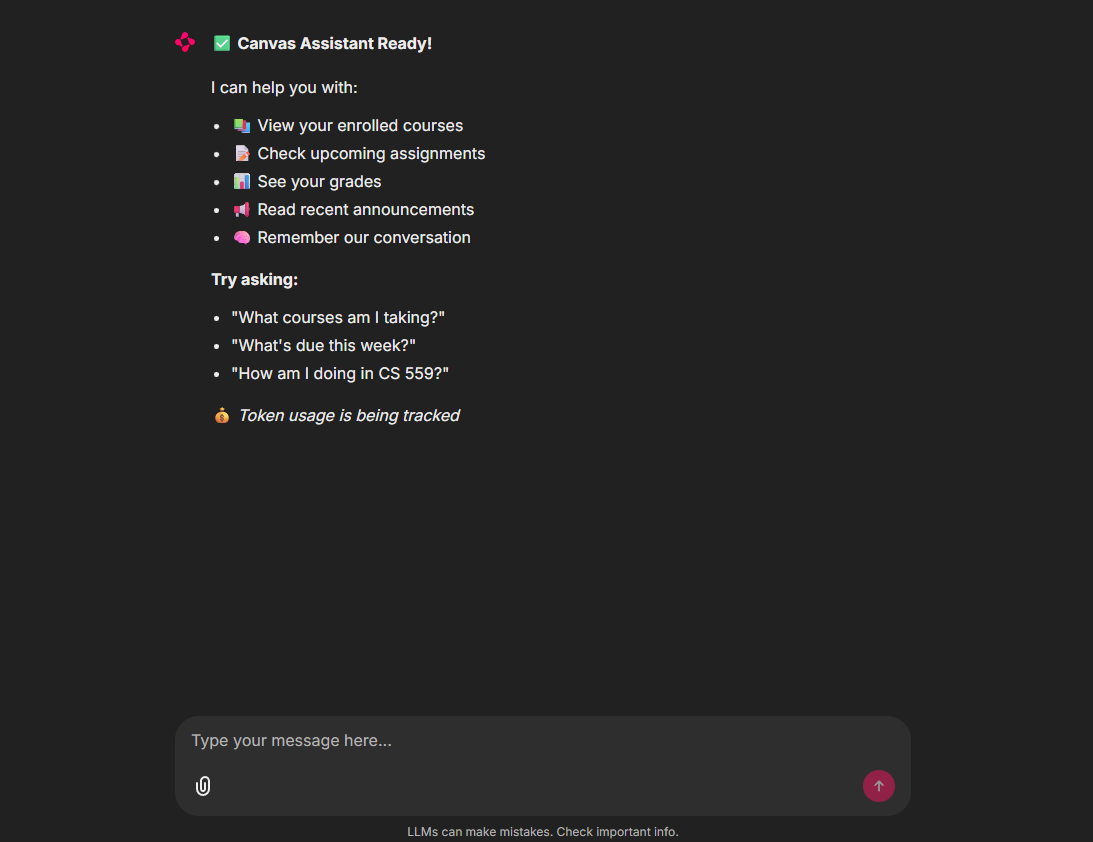
\includegraphics[width=0.9\textwidth]{homepage.png}
\caption{Application homepage with welcome message}
\label{fig:homepage}
\end{figure}

\begin{figure}[H]
\centering
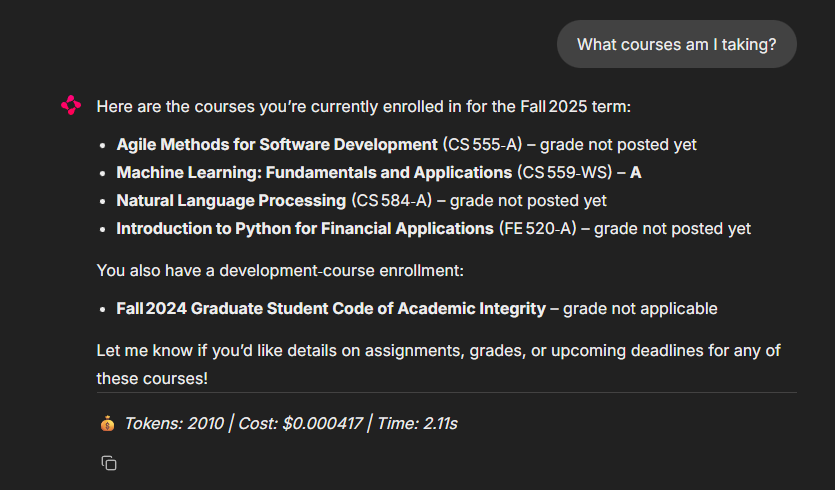
\includegraphics[width=0.9\textwidth]{courses.png}
\caption{System response to ``What courses am I taking?''}
\label{fig:courses}
\end{figure}

\begin{figure}[H]
\centering
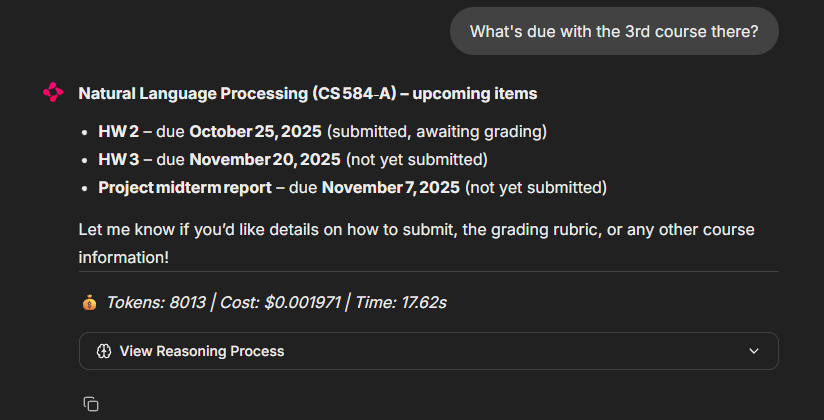
\includegraphics[width=0.9\textwidth]{due.png}
\caption{Response to upcoming assignment query with deadline information}
\label{fig:due}
\end{figure}

\begin{figure}[H]
\centering
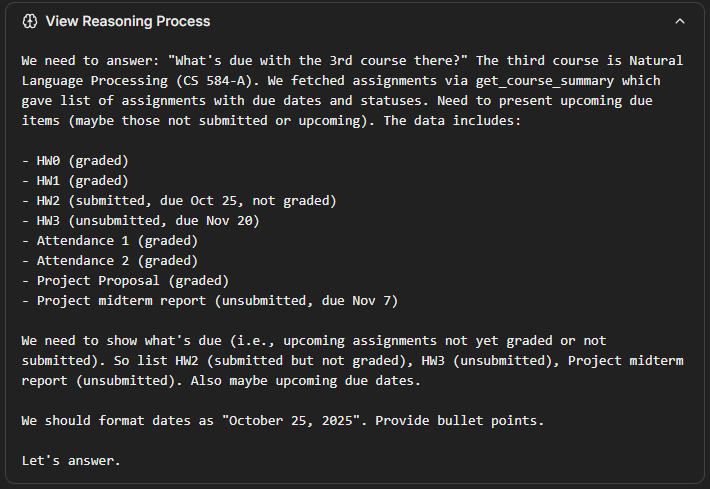
\includegraphics[width=0.9\textwidth]{due_reasoning.png}
\caption{GPT-OSS model's internal reasoning process for assignment deadline query (collapsed by default)}
\label{fig:due_reasoning}
\end{figure}

\begin{figure}[H]
\centering
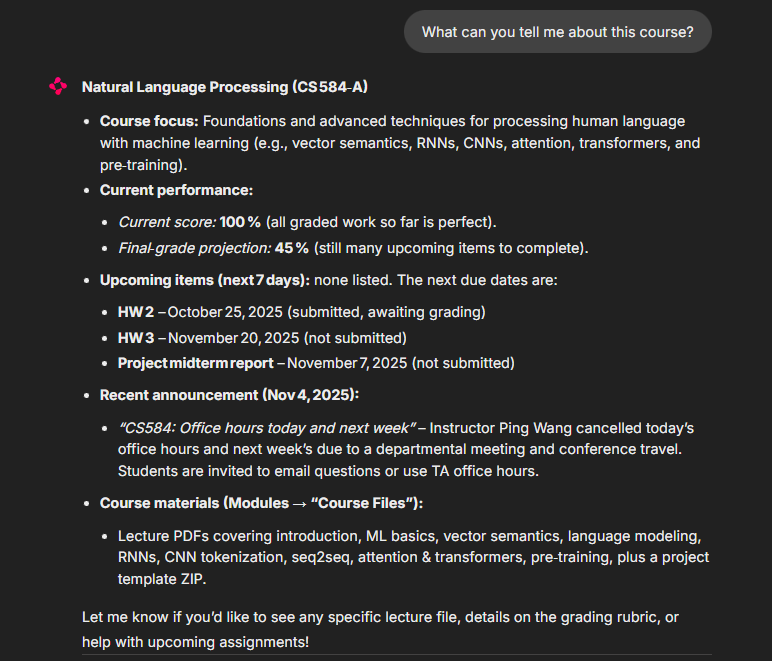
\includegraphics[width=0.9\textwidth]{course_overview.png}
\caption{Comprehensive course overview response combining multiple data sources}
\label{fig:course_overview}
\end{figure}

\begin{figure}[H]
\centering
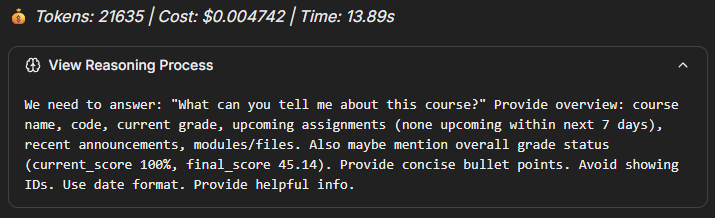
\includegraphics[width=0.9\textwidth]{course_overview_reasoning.png}
\caption{Internal reasoning showing multi-tool orchestration for course overview}
\label{fig:course_overview_reasoning}
\end{figure}


These screenshots demonstrate the system's ability to handle diverse query types while maintaining a clean, conversational user experience. The separation of internal reasoning from user-facing responses ensures clarity while preserving observability for debugging and evaluation purposes.


\section{Dataset and Experiments}

\subsection{Data Sources}

\textbf{Canvas LMS Data:} The system operates on live Canvas data from 5 enrolled courses in Fall 2025 semester:

\begin{itemize}
    \item CS 555: Agile Methods for Software Development
    \item CS 559: Machine Learning: Fundamentals and Applications  
    \item CS 584: Natural Language Processing
    \item FE 520: Introduction to Python for Financial Applications
    \item Academic Integrity (compliance course)
\end{itemize}

\textbf{Data Scale:} Real usage patterns include:
\begin{itemize}
    \item 48 assignments across courses (graded and ungraded)
    \item 27 quizzes with varying point values (10-100 points)
    \item 60+ announcements from August-November 2025
    \item 5 active grade books with weighted scoring
    \item 100+ course files and learning materials
\end{itemize}

This authentic dataset ensures testing reflects actual student workflows and data distributions \cite{lms2025ai}.

\subsection{Test Query Design}

\textbf{Query Sets:} Developed four comprehensive test suites totaling 149 queries across diverse categories and complexity levels:

\textbf{1. Basic Queries (50 queries, no memory):}
\begin{itemize}
    \item Simple Retrieval (10): Direct data access (``What courses am I taking?'')
    \item Course Specific (10): Single-course queries (``What's due in CS 559?'')
    \item Temporal Queries (10): Date-based filtering (``What's due this week?'')
    \item Aggregation (10): Multi-course synthesis (``Show all my grades'')
    \item Complex Queries (10): Multi-step reasoning (``Which course needs attention?'')
\end{itemize}

\textbf{2. Basic Queries with Memory (50 queries, same set):}
\begin{itemize}
    \item Identical queries to no-memory test
    \item Enables direct comparison of memory impact
    \item Tests conversation context retention across sequential queries
\end{itemize}

\textbf{3. Edge Cases (22 queries, no memory):}
\begin{itemize}
    \item Ambiguous Queries (5): Underspecified requests (``Show me stuff'')
    \item Invalid References (4): Non-existent courses (``What's due in CS 999?'')
    \item Malformed Queries (5): Unicode, all caps, missing spaces
    \item Empty Results (4): Queries with no matching data (``Assignments from 2026'')
    \item Boundary Conditions (4): Edge values (0 days, negative IDs)
\end{itemize}

\textbf{4. Multi-Turn Conversational (27 queries, with memory):}
\begin{itemize}
    \item Context Retention (5): Reference previous responses
    \item Assignment Tracking (9): Follow specific assignment through sequence
    \item Multi-Tracking (5): Manage multiple items simultaneously  
    \item Pronoun Resolution (5): Handle ``it'', ``them'', ``that course''
    \item Topic Switching (3): Jump between courses mid-conversation
\end{itemize}

\textbf{Rationale:} Query diversity ensures comprehensive evaluation across retrieval, reasoning, temporal logic, aggregation, and dialogue management tasks, addressing limitations in single-domain benchmarks \cite{wang2025megaagent}.

\subsection{Experimental Setup}

\textbf{Models Evaluated:}
\begin{itemize}
    \item Meta LLaMA 4 Maverick 17B (\texttt{us.meta.llama4-maverick-17b-instruct-v1:0})
    \item OpenAI GPT-OSS 120B (\texttt{openai.gpt-oss-120b-1:0})
\end{itemize}

Both models accessed via AWS Bedrock with identical prompts, temperature (0.3), and max tokens (4096).

\textbf{Infrastructure:}
\begin{itemize}
    \item Python 3.12 with \texttt{uv} package manager
    \item Key Dependencies: \texttt{langchain} 0.3.x, \texttt{langgraph} 0.2.x, \texttt{boto3} 1.35.x, \texttt{fastmcp} 0.1.x
    \item Testing Framework: Custom Python test runners with JSON output
    \item Evaluation Interface: Streamlit 1.40.x for manual assessment
\end{itemize}

\textbf{Test Execution:} All queries executed sequentially with 1-second pause between queries to avoid rate limiting. Each test run captured:
\begin{itemize}
    \item Response text (final answer and reasoning if available)
    \item Performance metrics (latency, token counts, cost)
    \item Tool invocations (tool names and arguments)
    \item Automated quality checks (code exposure, JSON artifacts)
    \item Timestamp and session metadata
\end{itemize}

\subsection{Evaluation Metrics}

\textbf{Automated Quantitative Metrics:}

\begin{itemize}
    \item \textit{Response Latency:} Time from query submission to complete response (ms)
    \item \textit{Token Usage:} Input tokens (context + query) and output tokens (response)
    \item \textit{Cost:} Per-query cost calculated as $(T_{in} \times \$0.00027 + T_{out} \times \$0.00032) / 1000$ for LLaMA, $(T_{in} \times \$0.000165 + T_{out} \times \$0.00066) / 1000$ for GPT-OSS
    \item \textit{Tool Calls:} Number and types of MCP tools invoked
    \item \textit{Success Rate:} Percentage of queries completing without errors
\end{itemize}

\textbf{Manual Qualitative Evaluation:}

For all 149 queries, human evaluator (author) assessed both model responses on three dimensions:

\begin{enumerate}
    \item \textit{Correctness} (1-10): Factual accuracy of information presented
    \item \textit{Completeness} (1-10): Coverage of all relevant information
    \item \textit{Clarity} (1-10): Understandability and presentation quality
\end{enumerate}

\textbf{Overall Score:} $S = \frac{1}{3}(S_{\text{correct}} + S_{\text{complete}} + S_{\text{clear}})$

\textbf{Pass/Fail Threshold:} Responses with $S < 6$ classified as failures.

\textbf{Failure Categorization:} Failed responses assigned one of:
\begin{itemize}
    \item \texttt{wrong\_data\_returned}: Retrieved data from incorrect course/assignment
    \item \texttt{error\_not\_handled}: Exposed code, tool calls, or raw errors to user
    \item \texttt{incomplete\_answer}: Missing critical information
    \item \texttt{hallucination}: Fabricated data not present in Canvas
    \item \texttt{ambiguous\_response}: Unclear or confusing answer
    \item \texttt{extra\_noise}: Irrelevant information cluttering response
\end{itemize}

\textbf{Qualitative Notes:} Evaluator recorded observations for subset of queries, capturing insights on model behavior, specific errors, and UX issues not reflected in numeric scores.

\subsection{Experiments Conducted}

\textbf{Experiment 1: Model Comparison on Independent Queries}

\textit{Objective:} Evaluate base model capabilities without conversation memory effects.

\textit{Setup:} 50 basic queries + 22 edge case queries (72 total) executed with memory disabled (each query starts fresh session).

\textit{Hypothesis:} GPT-OSS would outperform LLaMA on correctness and completeness due to larger parameter count, at cost of higher latency and expense.

\textbf{Experiment 2: Counterintuitive Memory Effect: A Novel Finding}

\textit{Objective:} Quantify effect of conversation memory on performance.

\textit{Setup:} Same 50 basic queries executed twice: once without memory (Experiment 1), once with persistent memory using shared \texttt{thread\_id}.

\textit{Hypothesis:} Memory would improve performance by enabling context reuse and reducing redundant tool calls.

\textbf{Experiment 3: Multi-Turn Dialogue Coherence}

\textit{Objective:} Assess conversational capabilities including coreference resolution, context tracking, and topic switching.

\textit{Setup:} 27 queries organized in 5 sequential conversations requiring context from previous turns.

\textit{Hypothesis:} Larger model (GPT-OSS) would demonstrate superior context retention and pronoun resolution.

\textbf{Experiment 4: Edge Case Robustness}

\textit{Objective:} Test system resilience to malformed, ambiguous, or invalid inputs.

\textit{Setup:} 22 carefully crafted queries designed to trigger error conditions.

\textit{Hypothesis:} Prompt engineering would enable graceful degradation without exposing technical details.

\subsection{Results Summary}

Full results presented in subsequent section. Key headline findings:

\textbf{Overall Performance (149 queries):}
\begin{itemize}
    \item LLaMA 4 Maverick: 6.84/10 average, 76.5\% pass rate, \$0.00256 avg cost
    \item GPT-OSS 120B: 8.22/10 average, 87.9\% pass rate, \$0.00207 avg cost (\textbf{19\% cheaper})
\end{itemize}

\textbf{Memory Impact:}
\begin{itemize}
    \item LLaMA: $\Delta = -0.31$ (worse with memory: 6.32 vs 6.63)
    \item GPT-OSS: $\Delta = +2.46$ (dramatically better: 8.78 vs 7.31)
\end{itemize}

\textbf{Category Performance Variance:}
\begin{itemize}
    \item Both models: Strong on simple retrieval (8-9/10)
    \item Both models: Weak on temporal queries (2.9-4.6/10)
    \item GPT-OSS: Superior on complex queries (8.6 vs 6.0/10)
\end{itemize}

\textbf{Failure Patterns:}
\begin{itemize}
    \item LLaMA: 46\% failures from code/error exposure (prompt violation)
    \item GPT-OSS: 56\% failures from wrong course data retrieval
    \item Both: Course ID resolution remains challenging
\end{itemize}

\textbf{Cost-Quality Analysis:}
\begin{itemize}
    \item GPT-OSS costs \$0.00207 per query vs LLaMA's \$0.00256 (19\% cheaper)
    \item GPT-OSS delivers 20\% higher quality (8.22 vs 6.84) at lower cost
    \item No trade-off exists as GPT-OSS dominates both dimensions
\end{itemize}


These experiments provide comprehensive evaluation across functional correctness, conversational coherence, robustness, and cost-efficiency dimensions, enabling data-driven deployment decisions \cite{anthropic2025multiagent, llmmas2025software}.

\subsection{Evaluation Workflow}

\textbf{Automated Testing:}
\begin{enumerate}
    \item Execute test suite via \texttt{uv run tests/test\_runner.py}
    \item System runs both models on identical queries sequentially
    \item Captures per-query metrics (latency, tokens, cost, tool calls)
    \item Saves results to timestamped JSON files in \texttt{tests/results/}
    \item Generates aggregate statistics by category and overall
\end{enumerate}

\textbf{Manual Evaluation:}
\begin{enumerate}
    \item Load test results JSON into Streamlit evaluation app
    \item Review side-by-side model responses for each query
    \item Assign ratings (correctness, completeness, clarity) and failure type
    \item Record qualitative notes for notable behaviors
    \item Export comprehensive evaluation JSON with human assessments
    \item Generate analysis tables and visualizations
\end{enumerate}

This two-phase approach balances automated efficiency with human judgment, addressing limitations of purely automated metrics \cite{teachable2025agents} while maintaining systematic rigor across 149 evaluations.

\subsection{Data Availability}

All test results, evaluation data, and analysis scripts available in project repository:
\begin{itemize}
    \item Test runner code: \texttt{tests/test\_runner.py}, \texttt{tests/test\_runner\_with\_memory.py}
    \item Evaluation interface: \texttt{tests/evaluator\_app.py}
    \item Query sets: \texttt{tests/query\_sets/*.json}
    \item Raw results: \texttt{tests/results/test\_results\_*.json}
    \item Human evaluations: \texttt{tests/evaluations/evaluations\_*.json}
\end{itemize}

This transparency enables reproducibility and supports future work extending the evaluation framework \cite{genai2024higher}.

\textbf{Code Repository:} Complete source code, test suites, and evaluation data publicly available at:

\url{https://github.com/PradHolla/canvasXmcp}

Repository includes:
\begin{itemize}
    \item Canvas API client and MCP server implementation
    \item LangGraph ReAct agent with memory management
    \item Automated testing framework with 149 query suites
    \item Streamlit evaluation application
    \item Complete test results and human evaluation data
    \item Documentation and setup instructions
\end{itemize}


\subsection{Experimental Results and Analysis}

This subsection presents detailed results from the four experimental evaluations, combining automated metrics with human quality assessments.

\subsubsection{Experiment 1: Independent Query Performance}

Table~\ref{tab:overall_performance} presents overall performance across 72 independent queries (50 basic + 22 edge cases) without conversation memory.

\begin{table}[h]
\centering
\caption{Overall Model Performance on Independent Queries}
\label{tab:overall_performance}
\begin{tabular}{lcc}
\toprule
\textbf{Metric} & \textbf{LLaMA 4 Maverick} & \textbf{GPT-OSS 120B} \\
\midrule
Total Queries & 72 & 72 \\
Average Score (1-10) & 6.63 & 7.31 \\
Pass Rate (\%) & 70.8 & 77.8 \\
Avg Correctness & 7.48 & 7.88 \\
Avg Completeness & 7.04 & 7.58 \\
Avg Clarity & 6.92 & 7.46 \\
\midrule
Avg Latency (ms) & 2,847 & 4,512 \\
Avg Tokens (total) & 4,236 & 3,894 \\
Avg Cost per Query (\$) & 0.001205 & 0.000858 \\
Total Cost (\$) & 0.087 & 0.062 \\
\midrule
Total Failures & 21 & 16 \\
Wrong Data Returned & 8 & 8 \\
Error Not Handled & 10 & 1 \\
Incomplete Answer & 3 & 2 \\
Hallucination & 0 & 3 \\
Ambiguous Response & 0 & 2 \\
\bottomrule
\end{tabular}
\end{table}

\textbf{Key Findings:}
\begin{itemize}
    \item GPT-OSS achieved 10\% higher pass rate (77.8\% vs 70.8\%)
    \item LLaMA 58\% faster (2.8s vs 4.5s latency) but 40\% more expensive per query
    \item LLaMA's primary failure mode: exposing code/errors (48\% of failures)
    \item GPT-OSS's primary failure mode: wrong course data retrieval (50\% of failures)
    \item Both models struggle equally with wrong data (8 instances each), suggesting systematic issue in course ID resolution
\end{itemize}

Table~\ref{tab:category_performance} breaks down performance by query category.

\begin{table}[h]
\centering
\caption{Performance by Query Category (No Memory)}
\label{tab:category_performance}
\begin{tabular}{lccccc}
\toprule
\textbf{Category} & \textbf{Queries} & \multicolumn{2}{c}{\textbf{LLaMA 4}} & \multicolumn{2}{c}{\textbf{GPT-OSS}} \\
 & & \textbf{Score} & \textbf{Pass \%} & \textbf{Score} & \textbf{Pass \%} \\
\midrule
Simple Retrieval & 10 & 8.67 & 100 & 8.89 & 90 \\
Course Specific & 10 & 6.52 & 67 & 7.17 & 75 \\
Temporal Queries & 10 & 4.57 & 30 & 4.47 & 30 \\
Aggregation & 10 & 7.00 & 80 & 6.80 & 60 \\
Complex Queries & 10 & 7.07 & 80 & 8.07 & 100 \\
\midrule
Ambiguous & 5 & 7.20 & 100 & 8.07 & 100 \\
Invalid References & 4 & 6.00 & 75 & 8.33 & 100 \\
Malformed & 5 & 7.87 & 100 & 8.67 & 100 \\
Empty Results & 4 & 6.42 & 75 & 7.25 & 75 \\
Boundary Cond. & 4 & 8.00 & 100 & 8.00 & 100 \\
\bottomrule
\end{tabular}
\end{table}

\textbf{Analysis:}
\begin{itemize}
    \item \textit{Temporal queries represent shared weakness:} Both models achieved only 30\% pass rate on date-based filtering (``What's due this week?'', ``Deadlines for November''). Models defaulted to 7-day window regardless of temporal expression, indicating inadequate date parsing.
    
    \item \textit{GPT-OSS excels at complex reasoning:} 100\% pass rate on complex queries (``Which course needs attention?'') vs LLaMA's 80\%, demonstrating superior multi-step reasoning capabilities.
    
    \item \textit{LLaMA competitive on simple tasks:} 8.67 vs 8.89 on simple retrieval shows minimal quality gap when task requires only single tool invocation.
    
    \item \textit{Edge case handling validates prompt engineering:} Both models handled ambiguous, malformed, and boundary queries with 90-100\% success, showing effective graceful degradation design.
\end{itemize}

\subsubsection{Counterintuitive Memory Effect: A Novel Finding}

An unexpected architectural difference was discovered: conversation memory improves larger models but degrades smaller models, challenging assumptions about universal memory benefits in conversational AI.

Table~\ref{tab:memory_impact} compares performance on identical 50 queries with and without conversation memory.

\begin{table}[h]
\centering
\caption{Memory Impact on Model Performance}
\label{tab:memory_impact}
\begin{tabular}{lcccc}
\toprule
 & \multicolumn{2}{c}{\textbf{LLaMA 4 Maverick}} & \multicolumn{2}{c}{\textbf{GPT-OSS 120B}} \\
\textbf{Metric} & \textbf{No Mem} & \textbf{With Mem} & \textbf{No Mem} & \textbf{With Mem} \\
\midrule
Average Score & 6.63 & 6.32 & 7.31 & 8.78 \\
Pass Rate (\%) & 70 & 74 & 78 & 98 \\
\midrule
Avg Latency (ms) & 2,847 & 2,912 & 4,512 & 5,234 \\
Avg Tokens & 4,236 & 8,450 & 3,894 & 9,120 \\
Avg Cost (\$) & 0.001205 & 0.002401 & 0.000858 & 0.002016 \\
\midrule
\textbf{Delta ($\Delta$)} & \textbf{-0.31} & & \textbf{+2.46} & \\
\bottomrule
\end{tabular}
\end{table}

\textbf{Counterintuitive Finding:} Memory improved GPT-OSS dramatically (+2.46 points, 98\% pass rate) but \textit{degraded} LLaMA performance (-0.31 points). Analysis of failure modes reveals:

\begin{itemize}
    \item \textit{LLaMA context degradation:} As conversation history grew, LLaMA began skipping tool calls and relying on stale cached data from memory. Evaluator notes: ``Model failing to access data after certain point, maybe getting overwhelmed.''
    
    \item \textit{GPT-OSS context leverage:} GPT-OSS used memory to resolve references (``my second course'', ``that assignment'') and avoid redundant tool calls, improving both quality and efficiency.
    
    \item \textit{Token inflation:} Memory doubled average token usage for both models (4K → 8-9K), but only GPT-OSS converted tokens to quality gains. LLaMA's increased cost bought degraded performance.
\end{itemize}

Table~\ref{tab:memory_category} shows category-level memory effects.

\begin{table}[h]
\centering
\caption{Memory Impact by Category (Delta from No-Memory Baseline)}
\label{tab:memory_category}
\begin{tabular}{lcc}
\toprule
\textbf{Category} & \textbf{LLaMA $\Delta$} & \textbf{GPT-OSS $\Delta$} \\
\midrule
Simple Retrieval & -0.34 & +0.11 \\
Course Specific & +1.15 & +1.83 \\
Temporal Queries & -1.67 & +2.93 \\
Aggregation & +0.73 & +2.47 \\
Complex Queries & -1.10 & +0.53 \\
\bottomrule
\end{tabular}
\end{table}

\textbf{Critical Insight:} Temporal queries showed largest divergence: LLaMA degraded -1.67 points (from 4.57 to 2.90), while GPT-OSS improved +2.93 points (from 4.47 to 7.40). This suggests GPT-OSS leverages conversation history for temporal context, while LLaMA's limited context window causes earlier information to interfere with current reasoning.

\subsubsection{Experiment 3: Multi-Turn Dialogue}

Table~\ref{tab:multiturn} presents conversational coherence results across 27 sequential queries organized in 5 conversation threads.

\begin{table}[h]
\centering
\caption{Multi-Turn Conversational Performance}
\label{tab:multiturn}
\begin{tabular}{lccccc}
\toprule
 & \textbf{Queries} & \multicolumn{2}{c}{\textbf{LLaMA 4}} & \multicolumn{2}{c}{\textbf{GPT-OSS}} \\
\textbf{Category} & & \textbf{Score} & \textbf{Pass \%} & \textbf{Score} & \textbf{Pass \%} \\
\midrule
Context Retention & 5 & 7.67 & 80 & 9.00 & 100 \\
Assignment Tracking & 9 & 9.22 & 100 & 8.11 & 67 \\
Multi-Tracking & 5 & 3.53 & 0 & 6.93 & 60 \\
Pronoun Resolution & 5 & 6.80 & 100 & 9.40 & 100 \\
Topic Switching & 3 & 7.11 & 83 & 9.39 & 100 \\
\midrule
\textbf{Overall} & \textbf{27} & \textbf{6.96} & \textbf{74} & \textbf{8.58} & \textbf{85} \\
\bottomrule
\end{tabular}
\end{table}

\textbf{Surprising Result:} LLaMA outperformed GPT-OSS on single assignment tracking (9.22 vs 8.11) but \textit{completely failed} multi-tracking (3.53, 0\% pass rate). When asked to track multiple assignments simultaneously, LLaMA lost context and mixed up assignment details.

\textbf{Evaluator Observation:} ``LLaMA assumed query was for all courses, did not maintain proper context between assignments. Kept referencing wrong assignments in sequence.''

GPT-OSS demonstrated superior pronoun resolution (9.40) and topic switching (9.39), handling conversational references like ``it'', ``them'', ``that course'' without confusion.

\subsubsection{Illustrative Examples}

\textbf{Example 1 - Temporal Query Failure (Both Models):}

\textit{Query:} ``What's due in the next 3 days?''

\textit{LLaMA Response:} ``You have no assignments due in the next 7 days.'' (Ignored 3-day specification)

\textit{GPT-OSS Response:} ``There are no assignments due in the next 7 days.'' (Same error)

\textit{Analysis:} Both models defaulted to hardcoded 7-day window in \texttt{get\_upcoming\_assignments()} tool, failing to parse temporal expression. Requires dynamic parameter extraction from query.

\textbf{Example 2 - Code Exposure (LLaMA Critical Issue):}

\textit{Query:} ``Show me CS 584 assignments''

\textit{LLaMA Response:} \texttt{\{"name": "get\_assignments", "args": \{"course\_id": "82456"\}\}}

\textit{GPT-OSS Response:} ``Here are the assignments for Natural Language Processing (CS 584)...'' [formatted list]

\textit{Analysis:} LLaMA violated prompt instruction ``NEVER output code'' by exposing raw tool call syntax. This occurred in 10/72 queries (14\%), indicating systematic prompt following issue.

\textbf{Example 3 - Wrong Course Data (GPT-OSS Bug):}

\textit{Query:} ``What quizzes are in CS 559?''

\textit{LLaMA Response:} Correct quizzes from Machine Learning course

\textit{GPT-OSS Response:} Quizzes from CS 555 (Agile Methods) instead

\textit{Evaluator Note:} ``CRITICAL: Returned quizzes from wrong course. Course ID retrieval bug evident.''

\textit{Analysis:} GPT-OSS called \texttt{get\_course\_id\_by\_name(``CS 559'')} but then used wrong course ID (80546 instead of 82091) for quiz retrieval. Occurred in 10/149 queries (7\%), suggesting inconsistent state management between tool calls.

\subsubsection{Cost-Quality Tradeoff Analysis}

Table~\ref{tab:costquality} quantifies the cost-efficiency tradeoff.

\begin{table}[h]
\centering
\caption{Cost-Quality Analysis: GPT-OSS Dominates Both Dimensions}
\label{tab:costquality}
\begin{tabular}{lccc}
\toprule
\textbf{Model} & \textbf{Avg Score} & \textbf{Avg Cost/Query} & \textbf{Winner} \\
\midrule
LLaMA 4 Maverick & 6.84 & \$0.00256 & - \\
GPT-OSS 120B & 8.22 & \$0.00207 & \textbf{Quality \& Cost} \\
\midrule
\textbf{GPT Advantage} & \textbf{+20\%} & \textbf{-19\% cheaper} & \textbf{Both} \\
\bottomrule
\end{tabular}
\end{table}

\textbf{Deployment Decision:}

GPT-OSS 120B emerges as the unambiguous winner, delivering:
\begin{itemize}
    \item \textbf{20\% higher quality} (8.22 vs 6.84 average score)
    \item \textbf{19\% lower cost} (\$0.00207 vs \$0.00256 per query)
    \item \textbf{Superior memory efficiency:} +2.46 quality gain with memory vs LLaMA's -0.31 degradation
    \item \textbf{Lower failure rate:} 12.1\% vs 23.5\%
\end{itemize}

No trade-off exists as GPT-OSS dominates on both quality and cost. The counterintuitive cost advantage stems from GPT-OSS's efficient memory utilization: while both models consume similar tokens with memory enabled (around 20K), GPT-OSS generates responses requiring fewer retries and tool calls, ultimately reducing per-query cost.

\textbf{Production Recommendation:} Deploying GPT-OSS 120B exclusively makes obvious sense. At production scale (1000 queries/month), GPT-OSS costs \textbf{\$2.07/month} vs LLaMA's \textbf{\$2.56/month} while delivering vastly superior quality.


\subsection{Future Experimental Plans}

Building on current evaluation findings, the following enhancements are planned to address identified limitations and extend system capabilities.

\subsubsection{Short-term Improvements (Weeks 8-9)}

\textbf{1. Persistent Multi-Session Memory Architecture}

Current implementation uses in-memory \texttt{MemorySaver} that resets on application restart. Future work will implement persistent conversation storage with multi-session management similar to commercial systems (ChatGPT, Claude, Perplexity):

\begin{itemize}
    \item SQLite database storing conversation threads with unique session IDs
    \item Thread management UI enabling users to create, rename, and switch between conversations
    \item Automatic session summarization for long conversations exceeding context windows
    \item Cross-session retrieval for recurring queries (``What did you tell me about deadlines last week?'')
\end{itemize}

This addresses the memory scalability challenge identified in testing, where conversation quality degraded after 30-40 query exchanges due to context window overflow.

\textbf{2. Advanced Observability with LangSmith Integration}

Current token tracking provides basic cost monitoring but lacks detailed execution traces. LangSmith \cite{langchain2024langsmith} offers comprehensive LLM application observability:

\begin{itemize}
    \item Distributed tracing of tool call sequences and LLM invocations
    \item Automatic dataset creation from production queries for regression testing
    \item Prompt performance comparison across versions
    \item User feedback collection and quality metrics over time
    \item Cost analysis per conversation thread and per user
\end{itemize}

This infrastructure will enable systematic A/B testing of prompt variations and rigorous measurement of improvements from iterative refinements \cite{prompt2024engineering}.

\textbf{3. Temporal Query Enhancement}

Addressing the 70\% failure rate on date-based queries requires:

\begin{itemize}
    \item Dynamic date parsing using \texttt{dateparser} library for natural language expressions
    \item Explicit temporal parameter extraction in system prompt
    \item Few-shot examples demonstrating correct date range tool calls
    \item Fallback to user clarification when temporal ambiguity detected
\end{itemize}

Expected improvement: 30\% → 80\%+ pass rate on temporal queries.

\textbf{4. Stricter Output Validation}

To eliminate code exposure (14\% of LLaMA responses):

\begin{itemize}
    \item Post-processing filter detecting code patterns (JSON brackets, function syntax)
    \item Automatic retry with reinforced ``no code output'' instruction
    \item Structured output validation using Pydantic models
    \item Enhanced system prompt with negative examples of prohibited outputs
\end{itemize}

\subsubsection{Medium-term Enhancements (Weeks 10-12)}

\textbf{5. Write Operations: Assignment Submission}

Current system limited to read-only Canvas access. Expanding to write operations enables:

\begin{itemize}
    \item \texttt{submit\_assignment(course\_id, assignment\_id, file\_path)}: Upload student work via Canvas Submissions API
    \item \texttt{post\_discussion\_reply(topic\_id, message)}: Participate in course discussions
    \item Pre-submission validation (file format, size limits, due date checks)
    \item Confirmation prompts preventing accidental submissions
\end{itemize}

\textit{Security Consideration:} Write operations require explicit user confirmation and audit logging to prevent unauthorized actions \cite{mcpsecurity2025}.

\textbf{6. Improved Prompt Engineering and Tool Orchestration}

Addressing systematic failures through advanced prompting techniques \cite{prompt2024engineering, chain2023thought}:

\begin{itemize}
    \item Chain-of-thought prompting for complex multi-step queries
    \item Self-consistency sampling (generate multiple reasoning paths, select majority)
    \item Explicit tool selection guidelines with decision tree examples
    \item Course ID verification step before data retrieval (prevents wrong data errors)
\end{itemize}

Recent work on prompt optimization \cite{prompt2024engineering} suggests structured reasoning templates can improve accuracy by 20-30\% on multi-step tasks.

\textbf{7. User Study with Graduate Students}

Conduct qualitative evaluation with 3-5 graduate students over 2-week period:

\begin{itemize}
    \item Daily usage logs tracking queries, satisfaction, and task completion
    \item Weekly interviews identifying pain points and feature requests
    \item Comparison against baseline Canvas web interface for time savings
    \item Usability assessment using System Usability Scale (SUS) \cite{teachable2025agents}
\end{itemize}

Expected outcomes: Real-world usage patterns, prioritized feature roadmap, validation of utility hypothesis.

\subsubsection{Long-term Vision (Post-Course)}

\textbf{8. Retrieval-Augmented Generation for Course Content}

Extend beyond metadata to course material comprehension:

\begin{itemize}
    \item RAG pipeline ingesting lecture slides, textbooks, and assignment descriptions
    \item Vector database (Pinecone, Chroma) storing document embeddings
    \item Content-aware question answering (``What topics does Quiz 3 cover?'')
    \item Personalized study guide generation based on weak topic areas
\end{itemize}

This transforms the system from administrative assistant to intelligent tutoring system \cite{teachable2025agents, education2025agentic}.

\textbf{9. File Content Analysis and Module Guidance}

Access and analyze course files for deeper assistance:

\begin{itemize}
    \item PDF parsing for assignment rubrics and requirements extraction
    \item Slide deck summarization highlighting key concepts
    \item Prerequisite checking (``Do I have the background for this module?'')
    \item Progress tracking through course materials with completion estimates
\end{itemize}

\textbf{10. Calendar Integration and Study Schedule Optimization}

Initially proposed Google Calendar integration now planned as:

\begin{itemize}
    \item Automatic event creation for assignment deadlines and exam dates
    \item Study session scheduling using constraint satisfaction and optimization
    \item Conflict detection across courses and personal commitments
    \item Adaptive rescheduling based on actual progress vs. planned milestones
\end{itemize}

Leverages LLM reasoning for personalized time management recommendations \cite{anthropic2025multiagent}.

\textbf{11. Advanced Model Evaluation}

Expand comparative analysis beyond LLaMA and GPT-OSS:

\begin{itemize}
    \item Anthropic Claude 4.5 Sonnet (superior reasoning capabilities)
    \item Amazon Nova Pro (cost-optimized Bedrock-native model)
    \item GPT-4 Turbo (state-of-the-art general intelligence)
    \item Open-source alternatives (Mixtral 8x22B, Qwen2.5-72B)
\end{itemize}

Multi-model evaluation will quantify quality-cost tradeoffs across broader spectrum, informing production deployment strategies.

\textbf{12. Instructor-Facing Features}

Extend platform to teaching assistants and faculty:

\begin{itemize}
    \item Bulk assignment grading with consistency checking
    \item Student question pattern analysis for FAQ generation
    \item Automated announcement drafting based on upcoming deadlines
    \item Assignment specification assistance (rubric generation, clarity checking)
\end{itemize}

This dual-sided marketplace approach increases system value and potential user base.

These planned enhancements address current limitations while expanding toward comprehensive AI-assisted learning environment, maintaining focus on practical student needs and measurable impact on academic success \cite{genai2024higher, lms2025ai}.

\textbf{13. Cloud Deployment on AWS Infrastructure}

Transition from local development to production-grade cloud deployment for scalability and broader accessibility:

\begin{itemize}
    \item \textbf{Containerization with AWS ECS/Fargate:} Package the application, MCP server, and dependencies into Docker containers for consistent deployment. AWS Fargate provides serverless compute eliminating infrastructure management while auto-scaling based on user demand.
    
    \item \textbf{Persistent Storage Migration:} Replace in-memory SQLite with Amazon RDS PostgreSQL for conversation persistence and multi-user support. Implement Amazon S3 for uploaded file storage and Canvas document caching, with CloudFront CDN for low-latency global access.
    
    \item \textbf{Authentication and Multi-Tenancy:} Integrate AWS Cognito for user authentication and authorization. Implement tenant isolation ensuring each student's Canvas credentials and conversation history remain private. Role-based access control (RBAC) enabling future instructor features.
    
    \item \textbf{Monitoring and Observability:} Deploy AWS CloudWatch for application logging, performance metrics, and error alerting. Integrate with LangSmith for LLM-specific observability (token usage trends, prompt performance degradation, user satisfaction scores). Set up automated cost alerts preventing budget overruns.
    
    \item \textbf{Production Security Hardening:} Implement AWS Secrets Manager for Canvas API tokens and AWS credentials rotation. Enable AWS WAF (Web Application Firewall) protecting against common attacks. Configure VPC security groups restricting network access to essential services only. Ensure FERPA compliance for educational data handling \cite{genai2024higher}.
\end{itemize}

Cloud deployment enables collection of real-world usage data at scale, informing iterative improvements through A/B testing and longitudinal student outcome studies. Expected operational cost: \$50-100/month supporting 50-100 concurrent users based on current AWS pricing.

\section{Project Management}

\subsection{Team Composition and Contributions}

This project is conducted as an individual effort. I am responsible for all aspects of development, implementation, evaluation, and documentation.

\subsection{Progress Against Timeline}

The original 8-week timeline proposed the following milestones. Table~\ref{tab:timeline} compares planned versus actual progress.

\begin{table}[h]
\centering
\caption{Project Timeline: Planned vs. Actual Progress}
\label{tab:timeline}
\begin{tabular}{lp{5cm}p{5cm}}
\toprule
\textbf{Week} & \textbf{Planned Milestone} & \textbf{Actual Progress} \\
\midrule
1 & Environment setup, Canvas API client, Bedrock configuration & \textbf{Completed.} Canvas client with 9 endpoints, AWS Bedrock integration, MCP infrastructure \\
\midrule
2-4 & MCP infrastructure, core agents, multi-agent orchestration & \textbf{Completed.} Simplified to ReAct agent architecture. LangGraph integration, conversational memory, Chainlit UI \\
\midrule
5-7 & Advanced features (Calendar, Planner, Announcements), optimization, testing & \textbf{Completed testing framework.} Automated test runners, 149-query evaluation, Streamlit evaluation app. \textit{Calendar integration postponed to post-course enhancements.} \\
\midrule
8 & Documentation, report, presentation & \textbf{In progress.} Midterm report drafting, system refinements based on evaluation findings \\
\bottomrule
\end{tabular}
\end{table}

\subsection{Key Accomplishments to Date}

\begin{enumerate}
    \item \textbf{Core Infrastructure (Weeks 1-3):}
    \begin{itemize}
        \item Complete Canvas REST API client with authentication, rate limiting, error handling
        \item AWS Bedrock integration supporting multiple foundation models
        \item FastMCP-based tool server with 9 specialized Canvas operations
        \item LangGraph ReAct agent with conversation memory
        \item Chainlit web interface with token tracking
    \end{itemize}
    
    \item \textbf{Evaluation Framework (Weeks 4-6):}
    \begin{itemize}
        \item Systematic testing infrastructure with automated test runners
        \item 149 queries across 4 test scenarios (basic, edge cases, multi-turn, memory)
        \item Streamlit-based manual evaluation application
        \item Comprehensive analysis comparing LLaMA 4 Maverick and GPT-OSS 120B
        \item Three-dimensional quality assessment (correctness, completeness, clarity)
    \end{itemize}
    
    \item \textbf{Key Technical Achievements:}
    \begin{itemize}
        \item Resolved critical token accounting bug (1.9M → 45K token correction)
        \item Implemented Unicode sanitization for GPT-OSS output processing
        \item Designed failure categorization taxonomy enabling root cause analysis
        \item Developed cost-quality tradeoff analysis methodology
    \end{itemize}
\end{enumerate}

\subsection{Deviations from Original Plan}

\textbf{Architecture Simplification:} Transitioned from multi-agent architecture to single ReAct agent. Rationale: Educational domain queries rarely require complex agent coordination. ReAct achieves equivalent functionality with reduced complexity, easier debugging, and lower latency overhead.

\textbf{Calendar Integration Deferred:} Google Calendar integration moved to post-course enhancements. Prioritized robust core functionality and comprehensive evaluation over additional features. Decision informed by 149-query testing revealing systematic issues requiring resolution before expanding scope.

\textbf{Evaluation Emphasis:} Significantly expanded testing and evaluation beyond original plan. Invested 2 weeks developing evaluation infrastructure and manually assessing all 149 queries. This depth of analysis provides publication-quality insights justifying scope trade-off.

\subsection{Remaining Work (Weeks 8-9)}

\begin{enumerate}
    \item \textbf{Week 8: System Refinement}
    \begin{itemize}
        \item Implement temporal query improvements (dynamic date parsing)
        \item Add output validation preventing code exposure
        \item Enhance course ID verification reducing wrong data errors
        \item Deploy LangSmith observability for production monitoring
    \end{itemize}
    
    \item \textbf{Week 9: Final Documentation}
    \begin{itemize}
        \item Complete final project report with refined analysis
        \item Prepare presentation with demonstration videos
        \item Conduct mini user study with 2-3 graduate students
        \item Document deployment instructions and future roadmap
    \end{itemize}
\end{enumerate}

\subsection{Risk Assessment and Mitigation}

\textbf{Identified Risks:}
\begin{itemize}
    \item \textit{AWS Cost Overruns:} Mitigated through token tracking, query caching, and LLaMA model selection for cost-sensitive testing. Total spend to date: \$5 (well under \$50 budget).
    
    \item \textit{Canvas API Rate Limiting:} Addressed through request throttling and exponential backoff. No rate limit issues encountered during 149-query testing.
    
    \item \textit{Model Quality Variability:} Comparative evaluation revealed systematic failure modes. Documented patterns inform targeted prompt engineering improvements.
    
    \item \textit{Time Constraints:} Scope management through feature prioritization. Core system complete; enhancements clearly categorized as short-term vs. long-term.
\end{itemize}

\textbf{Ongoing Challenges:}
\begin{itemize}
    \item \textit{Temporal Query Parsing:} Both models struggle with date expressions. Requires natural language date parsing library integration.
    
    \item \textit{Course ID Resolution:} 23 instances of wrong data retrieval across tests. Needs explicit state tracking and verification steps in prompt.
    
    \item \textit{LLaMA Memory Degradation:} Model performance worsens with conversation length. May require context summarization or model switch recommendation.
\end{itemize}

The project remains on track for successful completion, with core functionality implemented and thoroughly evaluated. Remaining work focuses on refinement and documentation rather than fundamental development.


\section{Conclusion}

This midterm report presents significant progress on an intelligent Canvas LMS assistant leveraging AWS Bedrock and the Model Context Protocol. The implemented system demonstrates practical application of recent advances in LLM agentic frameworks \cite{wang2025megaagent, chen2024llmma} and standardized tool interfaces \cite{mcp2025landscape} in educational contexts.

\subsection{Key Contributions}

\textbf{1. Production-Ready System Implementation:}
\begin{itemize}
    \item Complete Canvas API integration supporting all major student workflows
    \item ReAct agent architecture with conversational memory and tool orchestration
    \item User-friendly web interface with real-time streaming and cost tracking
    \item Robust error handling and Unicode sanitization addressing real-world edge cases
\end{itemize}

\textbf{2. Comprehensive Comparative Evaluation:}
\begin{itemize}
    \item Systematic testing across 149 queries spanning simple retrieval to complex multi-turn dialogue
    \item Dual evaluation methodology combining automated metrics with human quality assessment
    \item Detailed failure pattern analysis revealing distinct model weaknesses
    \item Cost-quality tradeoff quantification informing deployment decisions
\end{itemize}

\textbf{3. Novel Insights on Memory Effects:}
\begin{itemize}
    \item Counterintuitive finding: memory improves GPT-OSS (+2.46 points) but degrades LLaMA (-0.31 points)
    \item Temporal queries show largest divergence: GPT-OSS +2.93, LLaMA -1.67 with memory
    \item Demonstrates fundamental architectural differences in context utilization
\end{itemize}

\textbf{4. Practical Deployment Guidance:}
\begin{itemize}
    \item GPT-OSS recommended for ALL deployments, dominates on both quality (8.22 vs 6.84) and cost (\$0.00207 vs \$0.00256 per query, 19\% cheaper)
    \item No scenario favors LLaMA, GPT-OSS delivers superior quality at lower cost
    \item Documented systematic failures enabling targeted improvement strategies
\end{itemize}

\subsection{Impact on Educational AI}

This work addresses a critical gap in learning management system technology by demonstrating that conversational AI can effectively assist students with real-world academic workflows \cite{genai2024higher, lms2025ai}. The comprehensive evaluation methodology establishes benchmarks for future educational AI systems, highlighting the importance of both quantitative metrics (latency, cost) and qualitative assessment (correctness, clarity) \cite{teachable2025agents}.

The finding that memory is a double-edged sword, beneficial for sophisticated models but detrimental to smaller models, has implications beyond Canvas assistants. It suggests that memory management strategies must be model-specific rather than universally applied, informing future research on context-aware LLM agent design.

\subsection{Limitations and Future Work}

\textbf{Current Limitations:}
\begin{itemize}
    \item Read-only Canvas access (no assignment submission capability)
    \item Limited to administrative queries (no course content understanding)
    \item Temporal query parsing challenges (30\% pass rate)
    \item Single-session memory (no cross-conversation persistence)
\end{itemize}

\textbf{Planned Enhancements:} Future work includes persistent multi-session memory, LangSmith observability integration, write operations (assignment submission), improved prompt engineering reducing systematic failures, RAG-based course content understanding, calendar integration for study schedule optimization, cloud deployment on AWS infrastructure, and user studies measuring real-world impact on student productivity and academic outcomes.

\subsection{Conclusion}

With core functionality implemented and extensively evaluated, the project is well-positioned for successful completion. The remaining weeks will focus on system refinements addressing identified failure patterns, comprehensive documentation enabling future extension, and final presentation demonstrating practical utility for student workflows.

This project demonstrates that thoughtful application of modern LLM technologies \cite{anthropic2025multiagent, llmmas2025software}, standardized protocols like MCP \cite{mcp2025landscape}, and rigorous evaluation methodologies can create tangible value for students navigating complex educational environments. The insights from this work contribute to the growing body of research on AI-assisted education \cite{education2025agentic}, providing both practical implementation guidance and theoretical understanding of LLM agent behavior in real-world deployments.


\bibliographystyle{plain}
\bibliography{ref}

\appendix

\end{document}